\newpage
\section{17. 电话号码的字母组合}
\label{leetcode:17}

\subsection{题目}

给定一个仅包含数字 2-9 的字符串,返回所有它能表示的字母组合。

给出数字到字母的映射如下(与电话按键相同)。注意 1 不对应任何字母。

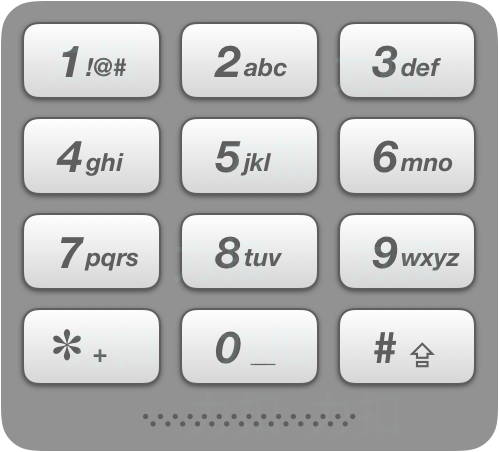
\includegraphics[width=50mm,height=50mm]{images/leetcode/17_telephone_keypad.png}

\textbf{示例}:

\begin{verbatim}
  输入:"23"
  输出:["ad", "ae", "af", "bd", "be", "bf", "cd", "ce", "cf"].
\end{verbatim}

\textbf{说明}: \\
尽管上面的答案是按字典序排列的,但是你可以任意选择答案输出的顺序。

\subsection{参考题解}

状态树如下,你只需要遍历整个树,把所有的叶子节点保存下来,
就是最终的结果。

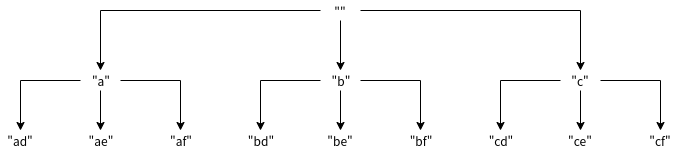
\includegraphics[width=150mm,height=40mm]{images/leetcode/leetcode_17.png}

\begin{verbatim}
/**
 * @param {string} digits
 * @return {string[]}
 */

const m = {
  '2': ['a', 'b', 'c'],
  '3': ['d', 'e', 'f'],
  '4': ['g', 'h', 'i'],
  '5': ['j', 'k', 'l'],
  '6': ['m', 'n', 'o'],
  '7': ['p', 'q', 'r', 's'],
  '8': ['t', 'u', 'v'],
  '9': ['w', 'x', 'y', 'z'],
};

var letterCombinations = function(digits) {
  if (digits.length === 0) { return []; }
  let result = [];
  dfs(result, "", digits);
  return result;
};

function dfs(result, node, digits) {
  if (digits.length === 0) {
    result.push(node);
    return;
  }
  let letters = m[digits[0]];
  for (let i = 0; i < letters.length; i += 1) {
    let letter = letters[i];
    dfs(result, node + letter, digits.substring(1));
  }
}
\end{verbatim}

\subsection{参考题解,分治回溯}

\begin{verbatim}
/**
 * @param {string} digits
 * @return {string[]}
 */
var letterCombinations = function(digits) {
  const m = {
    '2': ['a', 'b', 'c'],
    '3': ['d', 'e', 'f'],
    '4': ['g', 'h', 'i'],
    '5': ['j', 'k', 'l'],
    '6': ['m', 'n', 'o'],
    '7': ['p', 'q', 'r', 's'],
    '8': ['t', 'u', 'v'],
    '9': ['w', 'x', 'y', 'z'],
  };
  function recursion(digits) {
    if (digits.length === 0) {
      return [];
    }
    if (digits.length === 1) {
      return m[digits];
    }
    let result = [];
    let val = m[digits[0]];
    let sub = recursion(digits.substring(1));
    for (let i = 0; i < val.length; i += 1) {
      for (let j = 0; j < sub.length; j += 1) {
        result.push(val[i] + sub[j]);
      }
    }
    return result;
  }
  return recursion(digits);
};
\end{verbatim}
